\ifdefined\COMPLETE
\else
\documentclass[12pt]{article}
\usepackage{tikz}
\usetikzlibrary{shapes, calc, arrows, through, intersections, decorations.pathreplacing, patterns}



\begin{document}
\fi

\def\alph{$2+\sqrt{5}$}
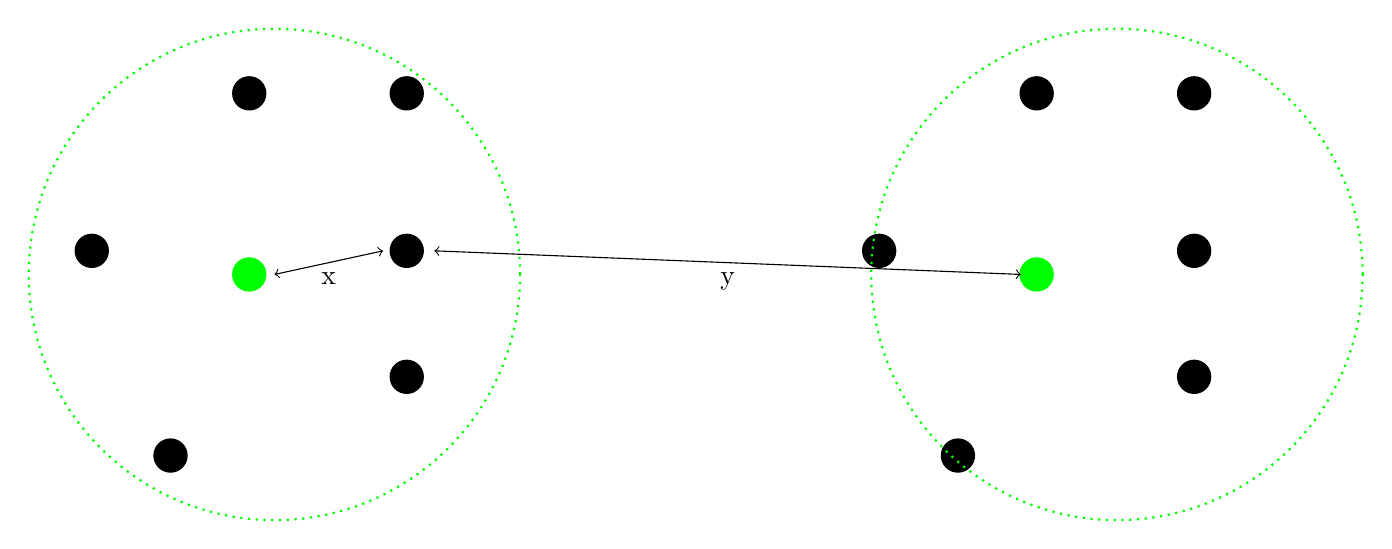
\begin{tikzpicture}
\filldraw[black] (3.0,2.3) circle (6pt) node[anchor=west] {};
\filldraw[black] (1.0,2.3) circle (6pt) node[anchor=west] {};
\filldraw[black] (3.0,0.3) circle (6pt) node[anchor=west] {};
\filldraw[black] (-1.0,0.3) circle (6pt) node[anchor=west] {};
\filldraw[black] (0.0,-2.3) circle (6pt) node[anchor=west] {};
\filldraw[black] (3.0,-1.3) circle (6pt) node[anchor=west] {};
\filldraw[green] (1.0,-0.0) circle (6pt) node[anchor=west] {};
\draw[green, thick, dotted] (1.32,0) circle (3.12);

\filldraw[black] (13.0,2.3) circle (6pt) node[anchor=west] {};
\filldraw[black] (11.0,2.3) circle (6pt) node[anchor=west] {};
\filldraw[black] (13.0,0.3) circle (6pt) node[anchor=west] {};
\filldraw[black] (9.0,0.3) circle (6pt) node[anchor=west] {};
\filldraw[black] (10.0,-2.3) circle (6pt) node[anchor=west] {};
\filldraw[black] (13.0,-1.3) circle (6pt) node[anchor=west] {};
\filldraw[green] (11.0,-0.0) circle (6pt) node[anchor=west] {};
\draw[green, thick, dotted] (12.02,0) circle (3.12);

\draw[<->](1.32, 0.0) -- node[below]{x} (2.7, 0.3);
\draw[<->](3.35, 0.3) -- node[below]{y} (10.8, 0.0);
\end{tikzpicture}

\begin{center}$\alpha x < y$\end{center}
\ifdefined\COMPLETE
\else
\end{document}
\fi
